% Filtro en el tiempo: sistema y cadena de verificación.
% Compilar: ver doc/diagramas/compilar.sh
\documentclass[tikz,border=8pt]{standalone}
\usepackage[T1]{fontenc}
\usepackage{lmodern}
\usepackage{amsmath}
\renewcommand{\familydefault}{\sfdefault}
\usetikzlibrary{arrows.meta,calc,positioning,fit}

\begin{document}
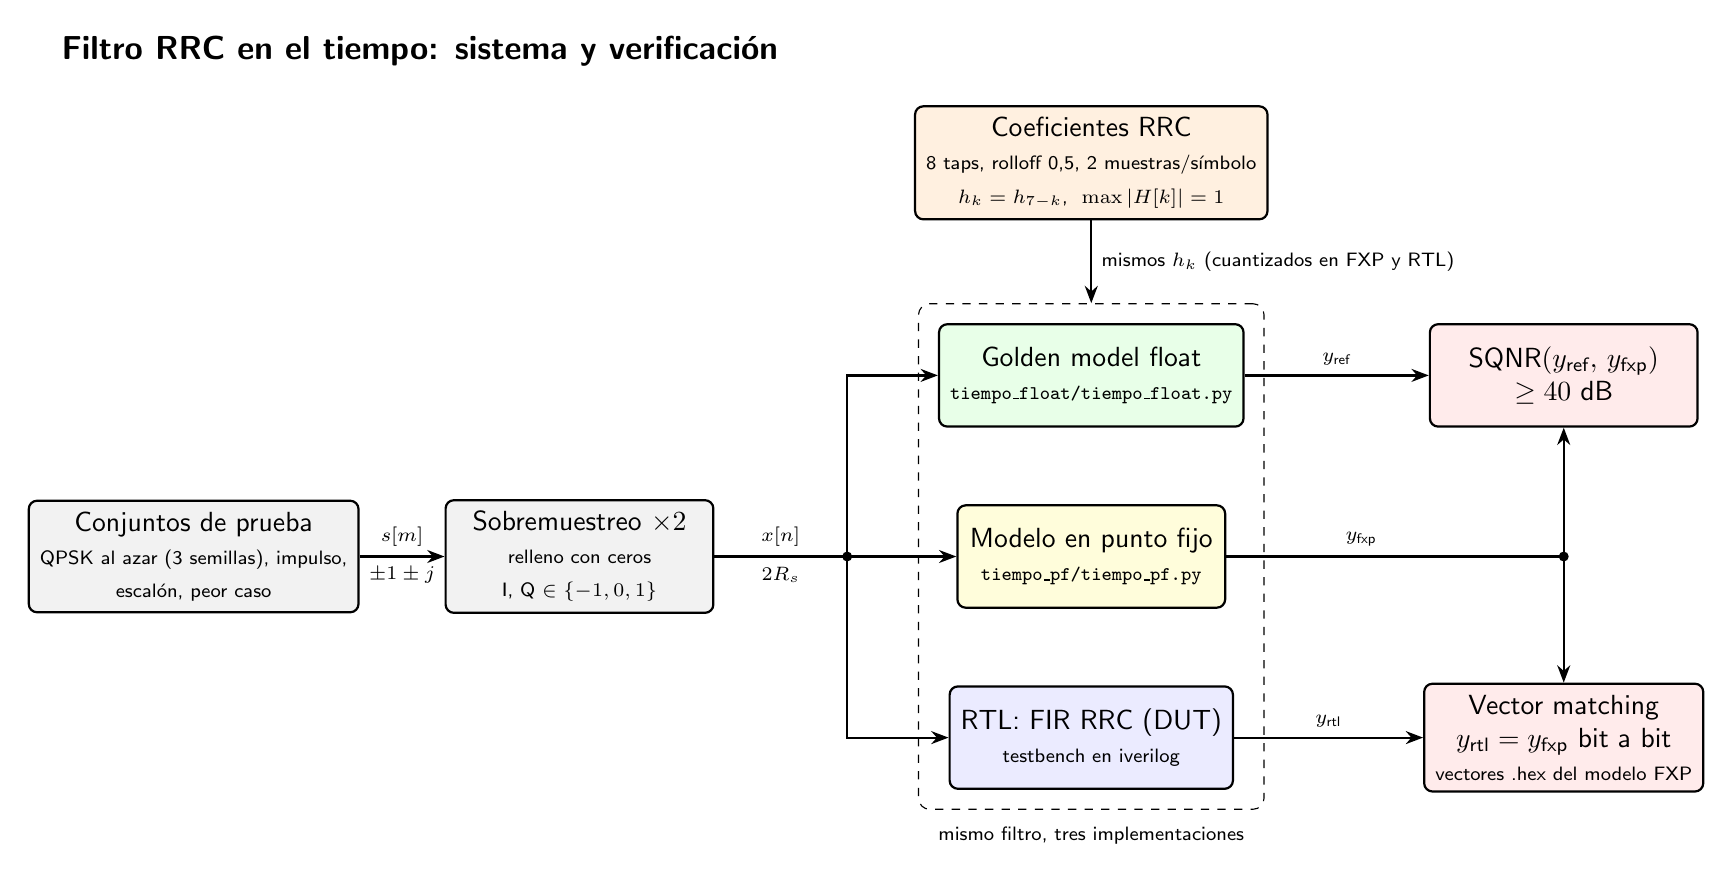
\begin{tikzpicture}[
  >={Stealth[length=2.2mm]},
  caja/.style={draw,thick,rounded corners=3pt,align=center,minimum height=13mm,
               minimum width=34mm,inner sep=4pt},
  etiq/.style={font=\scriptsize,align=center},
]

% ---------------- estímulo ----------------
\node[caja,fill=black!5] (gen) at (0,0)
  {Conjuntos de prueba\\ \scriptsize QPSK al azar (3 semillas), impulso,\\
   \scriptsize escalón, peor caso};
\node[caja,fill=black!5] (up) at (4.9,0) {Sobremuestreo $\times 2$\\ \scriptsize relleno con ceros\\ \scriptsize I, Q $\in\{-1,0,1\}$};
\draw[->,thick] (gen) -- node[etiq,above]{$s[m]$} node[etiq,below]{$\pm1\pm j$} (up);

% ---------------- tres implementaciones del mismo filtro ----------------
\node[caja,fill=green!9]  (flt) at (11.4,2.3)  {Golden model float\\ \scriptsize\texttt{tiempo\_float/tiempo\_float.py}};
\node[caja,fill=yellow!14] (fxp) at (11.4,0)    {Modelo en punto fijo\\ \scriptsize\texttt{tiempo\_pf/tiempo\_pf.py}};
\node[caja,fill=blue!8]   (rtl) at (11.4,-2.3) {RTL: FIR RRC (DUT)\\ \scriptsize testbench en iverilog};
\node[draw,dashed,rounded corners=4pt,fit=(flt)(fxp)(rtl),inner sep=7pt] (grupo) {};
\node[etiq,below=1mm of grupo] {mismo filtro, tres implementaciones};

\coordinate (bx) at (8.3,0);
\draw[thick] (up) -- node[etiq,above]{$x[n]$} node[etiq,below]{$2R_s$} (bx);
\fill (bx) circle (1.8pt);
\draw[->,thick] (bx) |- (flt.west);
\draw[->,thick] (bx) -- (fxp.west);
\draw[->,thick] (bx) |- (rtl.west);

% ---------------- coeficientes ----------------
\node[caja,fill=orange!12] (coef) at (11.4,5.0)
  {Coeficientes RRC\\ \scriptsize 8 taps, rolloff 0,5, 2 muestras/símbolo\\
   \scriptsize $h_k = h_{7-k}$, \ $\max|H[k]| = 1$};
\draw[->,thick] (coef) -- node[etiq,right]{mismos $h_k$ (cuantizados en FXP y RTL)} (grupo.north);

% ---------------- comparaciones ----------------
\node[caja,fill=red!8] (sq) at (17.4,2.3) {SQNR$(y_{\text{ref}},\,y_{\text{fxp}})$\\ $\geq 40$ dB};
\node[caja,fill=red!8] (vm) at (17.4,-2.3)
  {Vector matching\\ $y_{\text{rtl}} = y_{\text{fxp}}$ bit a bit\\ \scriptsize vectores .hex del modelo FXP};
\draw[->,thick] (flt.east) -- node[etiq,above]{$y_{\text{ref}}$} (sq.west);
\draw[->,thick] (rtl.east) -- node[etiq,above]{$y_{\text{rtl}}$} (vm.west);
\coordinate (bf) at (17.4,0);
\draw[thick] (fxp.east) -- node[etiq,above,pos=0.4]{$y_{\text{fxp}}$} (bf);
\fill (bf) circle (1.8pt);
\draw[->,thick] (bf) -- (sq.south);
\draw[->,thick] (bf) -- (vm.north);

\node[font=\large\bfseries,anchor=south west] at (-1.8,6.1)
  {Filtro RRC en el tiempo: sistema y verificación};
\end{tikzpicture}
\end{document}
